% Design Patterns for Data Structures
% Overleaf project: CoSc 320 Sort Paper Template
% File: paper-template.tex
% The LaTeX template for student papers in CoSc 320.
% !TEX TS-program = xelatex

\documentclass[10pt,fleqn]{article}

\usepackage{fontspec}
\usepackage{setspace}                        % For double spacing
\usepackage[slantedGreek]{mathptmx}          % For italic big-theta
\usepackage{amsmath,amssymb,amsfonts}        % Typical math resource packages
\usepackage{graphicx}                        % For inclusion of pdf graphics
\usepackage{booktabs}                        % For table rules
\usepackage{caption}
\usepackage{subcaption}                      % For side-by-side tables in figures
\usepackage[english]{babel}                  % For inserting blind text
\usepackage{blindtext}
\usepackage{hyperref}

\setmainfont{Times New Roman}

% Set spacing for table rows
%\renewcommand{\arraystretch}{1.5}

\title{A Comparison of Theoretical and Real Time Execution for Five Sorting Algorithms\\}
\author{Jason Press\\CoSc 320, Data Structures\\Pepperdine University}
\date{\today}

\begin{document}

\maketitle

% \onehalfspacing  % Provided by the setspace package

\begin{abstract}

The runtime performance of five sorting algorithms (Insertion Sort, Selection Sort, Heap Sort, Merge Sort, and Quick Sort) are compared to the theoretical runtime of each algorithm, and the practical runtime of each algorithm is compared to one another to determine the best sorting algorithm. Performance is measured by array element assignments and array element comparisons. 

\end{abstract}

\section{Introduction}

The Computer Science/Mathematics major at Pepperdine University focuses heavily on mathematics compared to other university's computer science courses. One drawback of this approach is that the theoretical runtime of algorithms is emphasized heavily, with less emphasis put on practical performance. There is only so far theory can go without being tested. This paper tests the theoretical performance of five sorting algorithms in the real world: Insertion Sort, Selection Sort, Heap Sort, Merge Sort, and Quick Sort.

Section 2 describes the methods used. Section 3 shows the raw data, followed by analysis of each sorting algorithm compared against itself, then against each other. Section 4 presents the conclusions.

\section{Methods}

Measuring the performance of the various sort algorithms might seem easy at first, but proves to be challenging. 

Using a timer might seem like an easy method to measure performance, as the runtime of the program is directly measured in real time. However, this brings up a lot of problems. First, all modern operating systems use some form of task scheduler, which rapidly switches between all active  tasks as to appear as if the operating system is running all active tasks at the same time. However, the central processing unit (CPU) can only execute one task at a time, so the scheduler assigns what tasks the CPU works on and in what order. This means that running the same program can have vastly differing real time runtimes based on the scheduler and other active background tasks, which is hard to make consistent from run to run \cite{dp4ds}.

Additionally, even if the task scheduler issue was somehow solved, different hardware architectures can cause different performance levels. Hardware is designed to conduct certain operations optimally. If a program is designed to take advantage of the hardware, it will have a better runtime on that hardware.

Optimization of C++ is handled by the compiler, which in my case is CMake, which itself has different levels of optimizations determined by the \verb|-O| flag. This means that even the same C++ code can be executed in a different amount of time based on how aggressively CMake optimizes the code: \verb|-O0| and \verb|-O3| C++ code can have different runtimes because of the compiler. All of the code executed in this paper was set to the same amount of CMake optimization.

Another option to measure performance is to measure the amount of CPU cycles that the program runs under, with the assumption that the amount of CPU cycles it takes to execute the program is proportional to the runtime. However, this is extremely hard to count \cite{dp4ds}.

Instead, this paper uses two different types of metrics that do not rely on runtime: the number of array element comparisons, and the number of array element assignments. Each method makes the assumption that the performance of the sort algorithms is directly proportional to the amount of times an operation on an array takes place \cite{dp4ds}. An array element assignment is anytime data is assigned to a cell of the array. An example in pseudo code may look like:

$$
\verb|array[index] = data;|
$$

An array element assignment is anytime data in a cell of the array is compared to another data type. An example in pseudo code may look like: 

$$
\verb|if (array[index] == data);|
$$

\subsection{Sort algorithms}

All of the sorting algorithms follow the Merritt sort taxonomy, which splits the list to be sorted into two smaller lists, sorts those, and then joins the sorted lists.

$\Theta(g.n)$ means that for some change in the size of the data $n$, the execution time changes by an amount $g.n$. This means the execution time of the function can be modelled approximately by the following function:

$$
    T(n) = \alpha_0 n^0+ \alpha_1 n^1 + . . . + \alpha_g g.n
$$

This is true for all $\Theta(g.n)$, where the execution time changes by an amount $g.n$. 

Some of the algorithms examined in this paper approach the fastest theoretical algorithm, which have a lower bound of $\Omega(n\lg n)$ \cite{dp4ds}: that is, the lowest possible $g.n$ is $n\lg n$.

The sort algorithms in this paper can be divided into two subsections: $\Theta(n\lg n)$ and $\Theta(n^2)$ algorithms.

\subsubsection{$\Theta(n\lg n)$ algorithms}

These algorithms are the Heap Sort, Merge Sort, and Quick Sort. These sorts are quick, but use up a lot of memory and are theoretically complicated. 

Quick Sort is "hard to split." When it splits, it splits the list such that the elements of first list are all less than or equal to the median value, and the elements of the second list are all greater than the median value. The median is determined by randomly sampling three values of the list and choosing the median of those. Then, the process is repeated on the two split lists. Joining is easy, with no code required, since the list is already sorted.

Merge Sort is "hard to join." When it splits, it just cuts the list in half. When it joins two lists, it puts the elements into a new array based on the size of elements in both lists, then copies that part to the location of where the two lists in the original array.

Heap Sort puts an array into max heap shape (called heapifying), swaps the root with the maximum element, splits the maximum element off, then sifts the root down to its location. It does this until the heap has a size of zero \cite{GeeksforGeeks_Heap}.

\subsubsection{$\Theta(n^2)$ algorithms}

These algorithms are Insertion Sort and Selection Sort. These sorts are easy to understand, but are computationally intensive and use less memory compared to their $\Theta(n \lg n)$ contemporaries.

Insertion Sort compares an element to its predecessor. If it's smaller, it swaps the elements, and repeats. Otherwise, it goes to the next unsorted element and repeats until the entire list is sorted. 

Selection Sort finds the maximum element in the list, swaps it with the last element, decreases the range by one, and repeats until the list is sorted. This is identical to Merge Sort, but the median value is the largest item in the list.

\subsection{Data collection}

Data for the array operations uses a \verb|CAMetrics| class, which has a \verb|_data| and a static counter for the type of operation. Whenever an operation with \verb|_data| is made, the counter for that type of operation is incremented by one. After the array is sorted, the overall count is returned.

The computer used to obtain results is a Samsumg 940X5N with an Intel Core i7-8550U CPU, with CMake version 3.25.1, running Debian 12. All of the code for the sorting algorithms is available from \url{https://github.com/TheRealCannedTuna/CoSc320SortPaperCode}

\subsection{Analysis}

Residual Standard Error (RSE) measures how good of a fit a least squares solution fits a given data sample. It follows this formula: 

\[
RSE =\sqrt{\frac{\sum{(y_i-\hat{y}_i)^2}}{d.f.}}
\]

where $y_i$ is the data value at $i$; $\hat{y_i}$ is the projection of $y_i$ onto the function being tested; $y_i-\hat{y}_i$ is the distance from the data point to the tested line; and $d.f$ is the number of degrees of freedom \cite{Choueiry_2020} . The data points being used are the number of array operations discussed earlier.

To determine if the algorithm fits its theoretical runtime, RSE will be calculated for both an $n\lg n$ and $n^2$ least squares fit. The least squares function that models the data the best will have the lowest RSE.

The best sorting algorithm is the one that is fastest and most stable.

\section{Results}

\subsection{Raw data}

Figure \ref{fig:assignment-plot} shows the number of assignments versus the size of the data to be sorted for all five sorting algorithms. Figure \ref{fig:comp-plot} shows the number of comparisons versus the size of the data to be sorted.

\begin{figure}[h]
\centering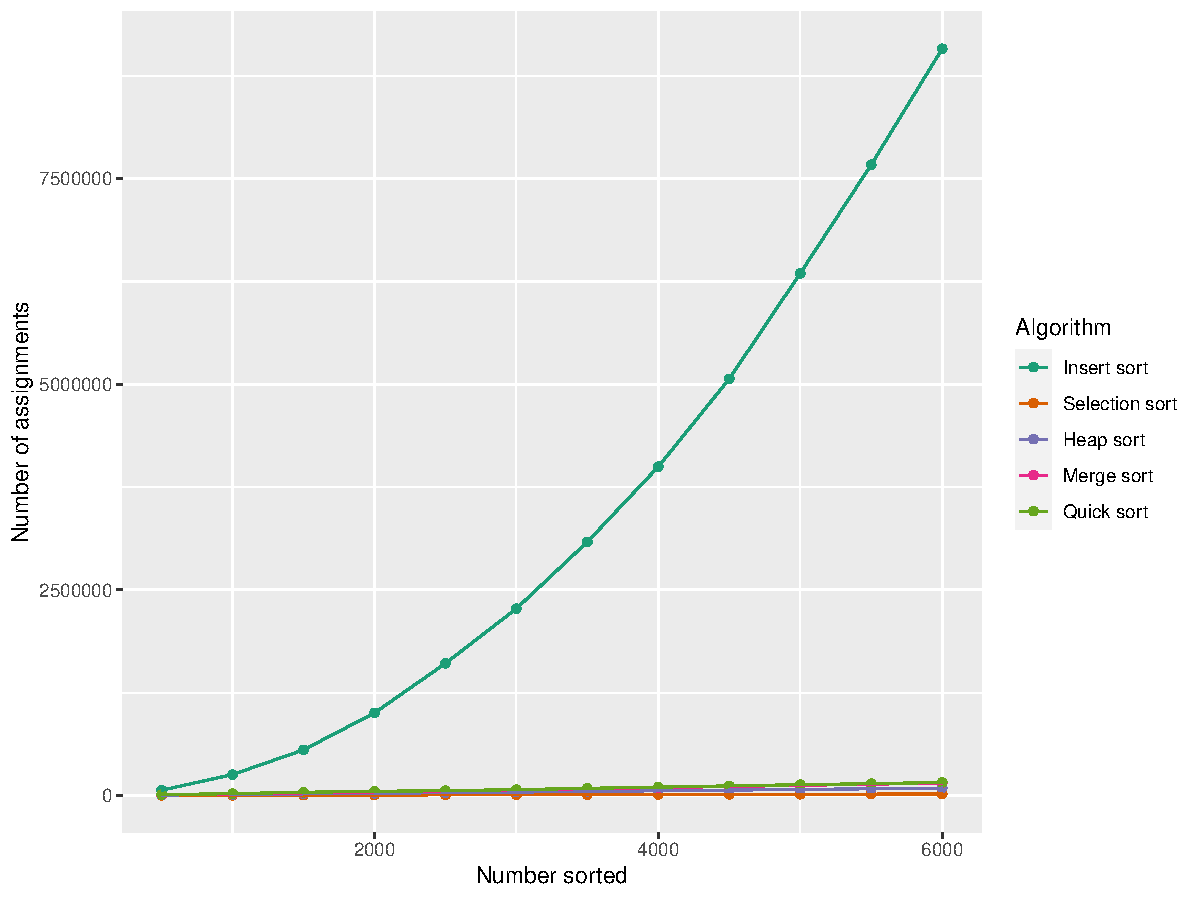
\includegraphics[scale=0.4]{CoSc 320 Sort Paper Template/assignment-plot.pdf}
\caption{Number of assignments versus size of data for all five sorting algorithms.}
\label{fig:assignment-plot}
\end{figure}

\begin{figure}[h]
\centering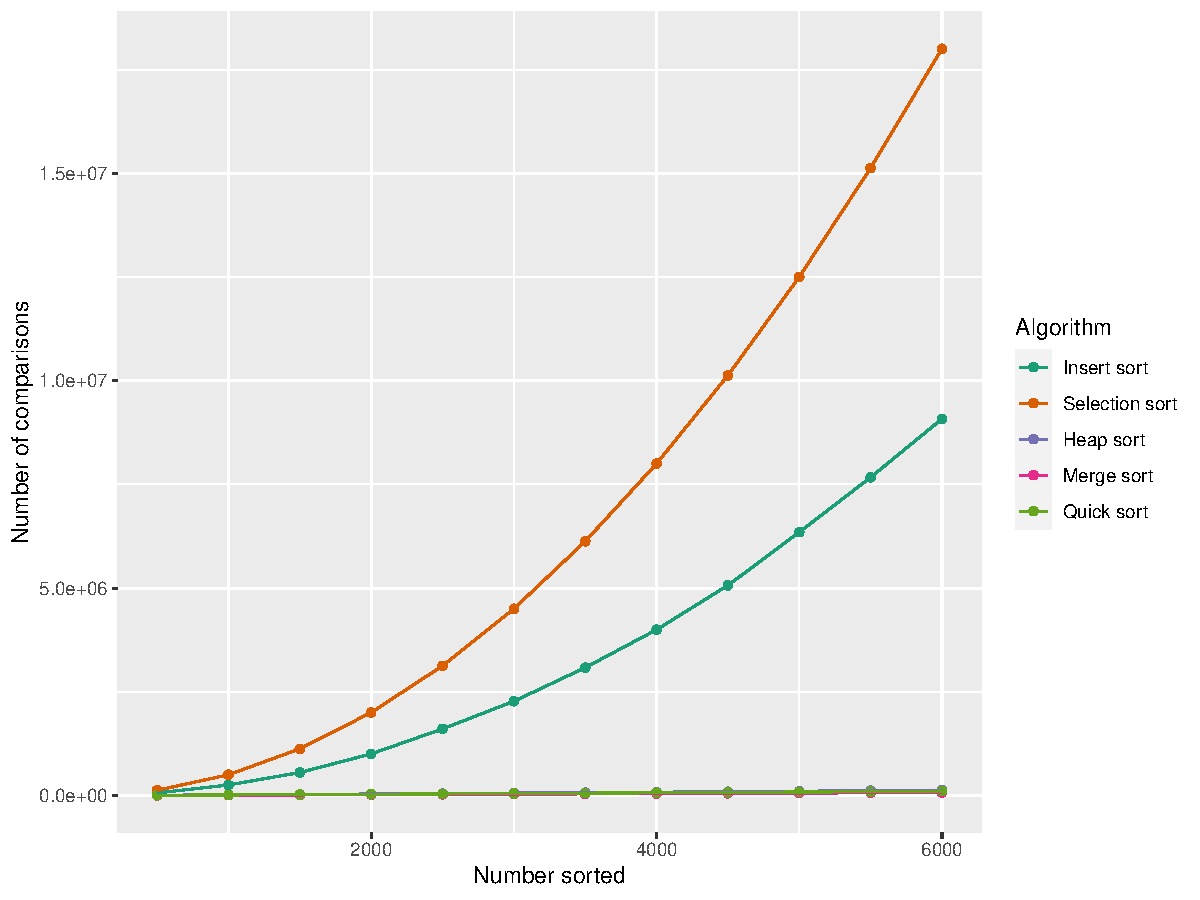
\includegraphics[scale=0.4]{CoSc 320 Sort Paper Template/comp-data-plot.pdf}
\caption{Number of comparisons versus size of data for all five sorting algorithms.}
\label{fig:comp-plot}
\end{figure}

Given the sheer amount of assignments and comparisons the $\Theta(n^2)$ algorithms have relative to the $\Theta(n\lg n)$ algorithms, plots of the raw data are not ideal for analysis. Instead, examining the data in table form is more useful. Figure \ref{fig:tableAsgn} shows the raw data for the number of assignments, Figure \ref{fig:assignment-plot} in table form. Figure \ref{fig:tableComp} shows the raw data for the number of comparisons, Figure \ref{fig:comp-plot} in table form.

\begin{figure}[h]
  \centering\begin{tabular}{ c | r r r r r }
  \toprule
  \sffamily\bfseries Number of   & \multicolumn{5}{c} {\sffamily\bfseries Algorithm} \\
  \sffamily\bfseries data points & Insert & Select &   Heap &  Merge &  Quick \\
  \midrule
        500 &        63604 &         1497 &       5667 &        8976 &      10450 \\
       1000 &       254367 &         2997 &      12335 &       19952 &      22146 \\
       1500 &       554593 &         4497 &      19415 &       31904 &      38996 \\
       2000 &      1003673 &         5997 &      26684 &       43904 &      50419 \\ 
       2500 &      1606137 &         7497 &      34207 &       56808 &      58494 \\
       3000 &      2272438 &         8997 &      41845 &       69808 &      70598 \\ 
       3500 &      3083561 &        10497 &      49556 &       82808 &      86881 \\
       4000 &      3997707 &        11997 &      57388 &       95808 &     101358 \\
       4500 &      5066605 &        13497 &      65354 &      109616 &     116648 \\
       5000 &      6349094 &        14997 &      73410 &      123616 &     131146 \\
       5500 &      7670593 &        16497 &      81442 &      137616 &     143529 \\
       6000 &      9080166 &        17997 &      89631 &      151616 &     158237 \\
  \bottomrule
  \end{tabular}
  \caption{Number of array element assignments.}
  \label{fig:tableAsgn}
\end{figure}

\begin{figure}[h]
  \centering\begin{tabular}{ c | r r r r r }
  \toprule
  \sffamily\bfseries Number of   & \multicolumn{5}{c} {\sffamily\bfseries Algorithm} \\
  \sffamily\bfseries data points & Insert & Select &   Heap &  Merge &  Quick \\
  \midrule
        500 &        63597 &       125249 &       7000 &        4344 &       6505 \\
       1000 &       254362 &       500499 &      15967 &        9700 &      14439 \\
       1500 &       554589 &      1125749 &      25813 &       15467 &      23090 \\
       2000 &      1003667 &      2000999 &      35962 &       21400 &      31188 \\
       2500 &      1606133 &      3126249 &      46662 &       27595 &      39061 \\
       3000 &      2272433 &      4501499 &      57608 &       33950 &      47481 \\
       3500 &      3083553 &      6126749 &      68686 &       40320 &      57100 \\
       4000 &      3997696 &      8001999 &      79945 &       46820 &      66042 \\
       4500 &      5066599 &     10127249 &      91547 &       53511 &      73877 \\
       5000 &      6349081 &     12502499 &     103334 &       60253 &      84645 \\
       5500 &      7670586 &     15127749 &     115147 &       66972 &      92018 \\
       6000 &      9080159 &     18002999 &     127042 &       73910 &     105180 \\

  \bottomrule
  \end{tabular}
  \caption{Number of array element comparisons.}
  \label{fig:tableComp}
\end{figure}

\subsection{Insertion sort}

Figure \ref{fig:assignment-plot} shows that Insertion Sort has by far the most amount of array assignments, and Figure \ref{fig:comp-plot} shows that Insertion Sort has the second most amount of array element comparisons.

For a quadratic fit on the number of comparisons, the RSE is 28130 on 9 degrees of freedom. For an $n \lg n$ fit, the RSE is 155300 on 9 degrees of freedom. 

For both the quadratic and $n\lg n$ fits, the RSE is the same for the number of array element assignments.

Therefore, Insertion Sort fits $\Theta(n^2)$ better than $\Theta(n\lg n)$, confirming the theoretical runtime of $\Theta(n^2)$. 

Visually, this can be seen in Figure \ref{fig:insert-plot} and \ref{fig:insert-plot-comp}, which shows both a least squares $n \lg n$ fit (in blue) and a least squares $n^2$ fit (in red) for the number of assignments and comparisons respectively. The $n^2$ least squares fit appears to fit the data better, which is backed up by the RSE.

\begin{figure}[h]
    \centering
    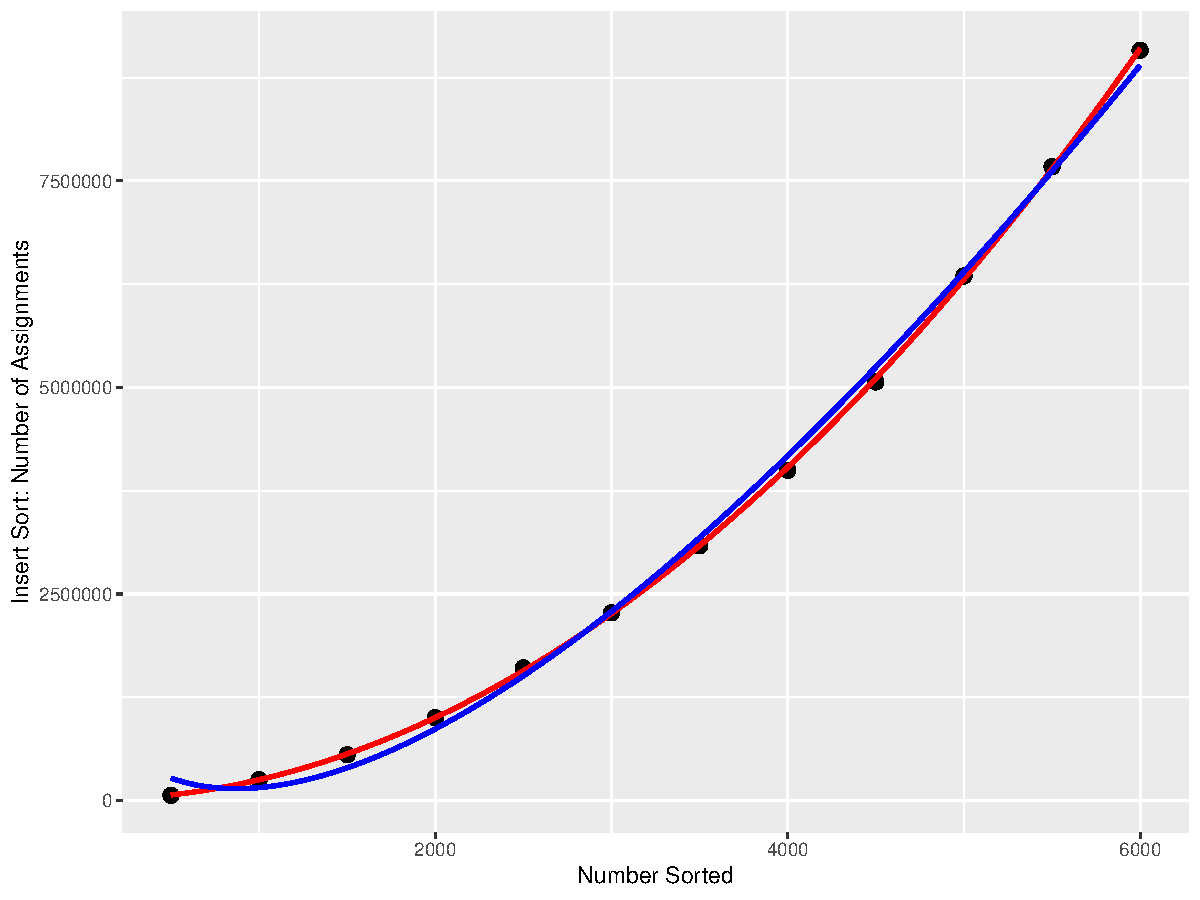
\includegraphics[scale=0.3]{CoSc 320 Sort Paper Template/insert-plot.pdf}
    \caption{$n^2$ and $n\lg n$ fit for the number of assignments for Insertion Sort.}
\label{fig:insert-plot}
\end{figure}

\begin{figure}[h]
    \centering
    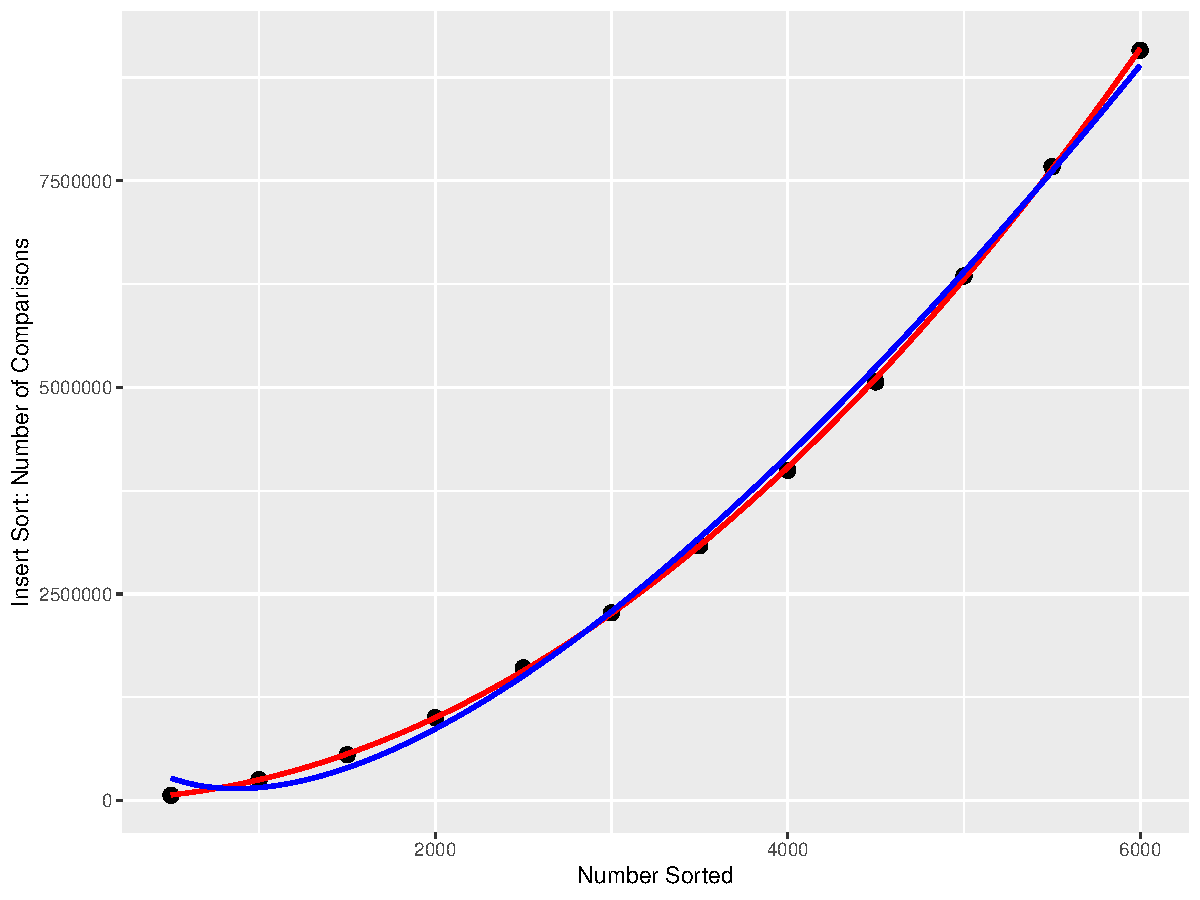
\includegraphics[scale=0.3]{CoSc 320 Sort Paper Template/insert-plot-comp.pdf}
    \caption{$n^2$ and $n\lg n$ fit for the number of comparisons for Insertion Sort.}
    \label{fig:insert-plot-comp}
\end{figure}

\subsection{Selection sort}

The examined algorithm for Selection Sort has by far the least amount of raw array element assignments, but by far the most amount of array element comparisons, as seen in Figure \ref{fig:tableAsgn} and Figure \ref{fig:tableComp}.

For the number of assignments, the RSE for the $n^2$ fit is $3.702\times10^{-12}$ on 9 degrees of freedom, and the RSE for the $n \lg n$ fit is $2.256\times10^{-12}$ on 9 degrees of freedom. Both of these numbers are so ridiculously small that they are more or less comparable. This makes sense, because the number of assignments is small.

For the number of comparisons, the RSE for the $n^2$ fit is $3.313\times10^{-9}$ on 9 degrees of freedom, and the RSE for the $n \lg n$ fit is $291500$ on 9 degrees of freedom. The RSE for the $n^2$ fit is dramatically lower than the $n \lg n$ fit. This confirms that Selection Sort is $\Theta(n^2)$, because the number of comparisons is dramatically larger than the number of assignments by three to four orders of magnitude. 

Figure \ref{fig:select-plot-comp} shows a least squares $n \lg n$ fit (in blue) and a least squares $n^2$ fit (in red) for the number of assignments and comparisons respectively. The $n^2$ least squares fit appears to fit the data better, which is backed up by the RSE.

\begin{figure}[h]
    \centering
    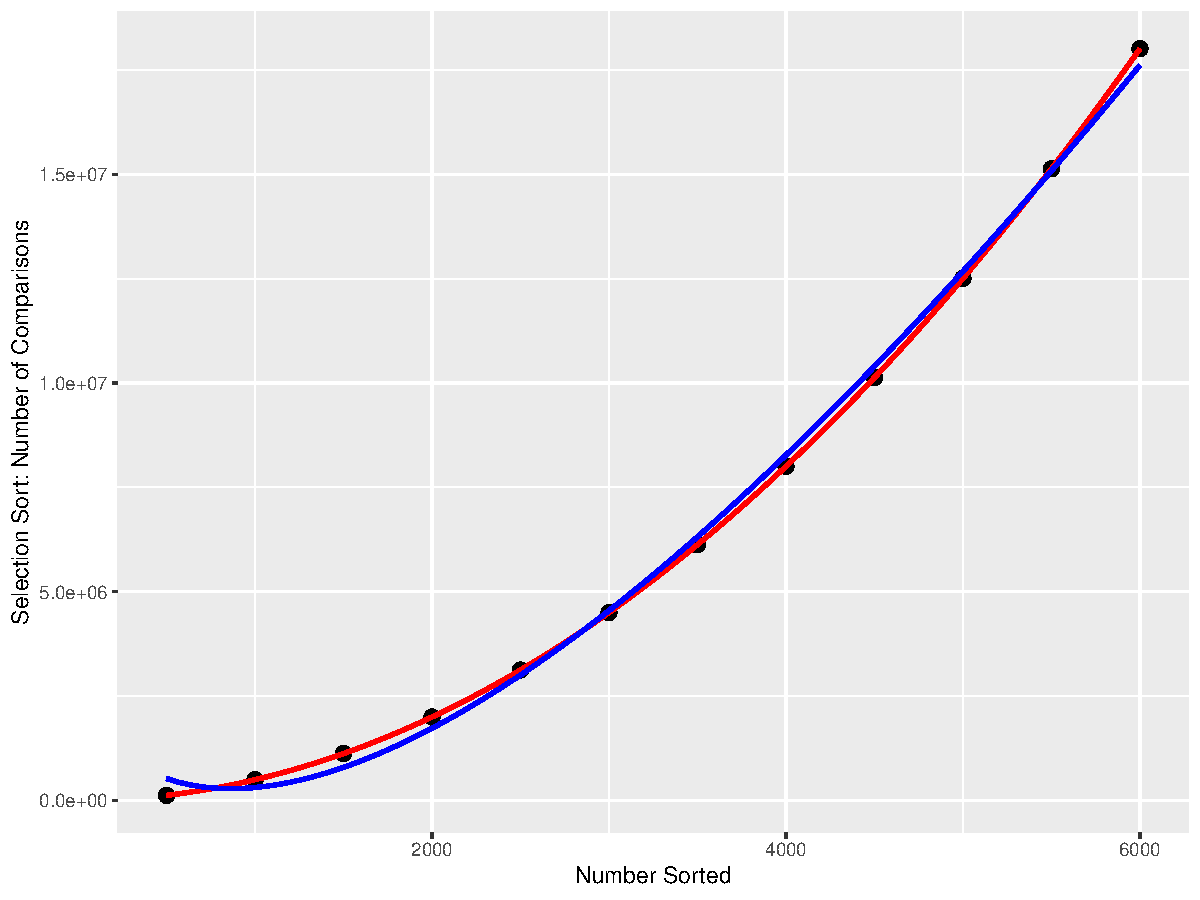
\includegraphics[scale=0.3]{CoSc 320 Sort Paper Template/select-plot-comp.pdf}
    \caption{$n^2$ and $n\lg n$ fit for the number of comparisons for Selection Sort.}
    \label{fig:select-plot-comp}
\end{figure}

\subsection{Heap sort}

Figure \ref{fig:tableAsgn} and \ref{fig:tableComp} show that Heap Sort has the most amount of array element comparisons with the least amount of array element assignments of the $n\lg n$ sort algorithms.

For the number of assignments, the RSE for the $n^2$ fit is $155.4$ on 9 degrees of freedom, and $22.41$ on 9 degrees of freedom for an $n\lg n$ fit. For the number of comparisons, the RSE for the $n^2$ fit is 312.9 on 9 degrees of freedom, and 56.79 on 9 degrees of freedom for an $n \lg n$ fit. This confirms that Heap Sort is $\Theta(n\lg n)$.

Since the RSE of both fits are so close, a graphical depiction of the fits is not useful for Heap Sort.

\subsection{Merge sort}

Figure \ref{fig:tableComp} show that Merge Sort the least amount of array element comparisons of the $n\lg n$ sort algorithms. Figure \ref{fig:tableAsgn} has substantially more assignments per amount of data than Heap Sort, but slightly less than the number of assignments for Quick Sort. 

For the number of assignments, the RSE for the $n^2$ fit is 291.8 on 9 degrees of freedom, and 190.1 on 9 degrees of freedom for an $n\lg n$ fit. For the number of comparisons, the RSE for the $n^2$ fit is 147.8 on 9 degrees of freedom, and 36.19 on 9 degrees of freedom for an $n \lg n$ fit. This confirms that Heap Sort is $\Theta(n\lg n)$.

Just like for Quick Sort, a graphical depiction of the fits is not useful for the same reasons.

\subsection{Quick sort}

Figure \ref{fig:tableComp} shows that Quick Sort has less comparisons than Heap Sort, but still more than Merge Sort. Figure \ref{fig:tableAsgn} shows that Quick Sort has marginally more assignments than Merge Sort, making it have the most amount of assignments of the $n\lg n$ sorting algorithms.

For the number of assignments, the RSE for the $n^2$ fit is 2193 on 9 degrees of freedom, but 2270 on 9 degrees of freedom for an $n\lg n$ fit. For the number of comparisons, the RSE for the $n^2$ fit is 928.5 on 9 degrees of freedom, but 1035 on 9 degrees of freedom for an $n \lg n$ fit.

Interestingly, the data is better fit by an $n^2$ curve, even though it is expected to be fit better by an $n\lg n$ curve, since Quick Sort is a $\Theta(n\lg n)$ algorithm. The reason for this is that the worst case scenario runtime for Quick Sort follows a function that is $\Theta(n^2)$, and the optimal case runtime is $\Theta(n\lg n)$. But Quick Sort is unstable, meaning order is not preserved in some cases (but not as bad as Heap Sort, discussed later), leading to a worse performance \cite{Musser1997IntrospectiveSA}. The random data samples means that Quick Sort varies between $\Theta(n^2)$ and $\Theta(n\lg n)$, since real world data is usually neither optimal nor worst case.

\subsection{Sort comparisons}

It is most useful to compare the $\Theta(n^2)$ sorting algorithms and $\Theta(n\lg n)$ sorting algorithms independently of each other, since the $\Theta(n^2)$ algorithms are both mathematically and practically slower than the $\Theta(n\lg n)$ sorting algorithms.

Assuming that array element assignments are equally as costly on performance as array element comparisons, both $\Theta(n^2)$ sorting algorithms are about equal in terms of performance: the number of array element assignments and array element comparisons combined for both sorting algorithms is about equal. However, it is worth noting that Selection Sort has the lowest amount of array element assignments per data point compared to all of the sorting algorithms.

The best $\Theta(n\lg n)$ algorithm is subjective. Quick Sort is great because it uses minimal memory while still managing to be significantly quicker than the $\Theta(n^2)$ algorithms in terms of assignments and comparisons combined. However, it is not as quick as Merge and Heap Sort because the worst case time complexity is $\Theta(n^2)$.

Heap Sort seems like the quickest sorting algorithm. However, Heap Sort is unstable because the list must be heapified before it is sorted. This means the array is sorted twice: one when heapified, and once after it is heapified. For lists that are already partially ordered, Heap Sort is not optimal, since heapifying does not preserve order.

Merge Sort is the last of the three $\Theta(n\lg n)$ algorithms. Its only drawback is that it is memory intensive compared to the other two sorting algorithms, because the elements of the array must be copied into a temporary array and back into the original array. Modern computer systems avoid this issue by having large amounts of memory: for example, the base model MacBook Air released in 2023 starts at "only" 8 GB of memory, more than 5,000 times the memory aboard the Saturn V.

\section{Conclusion}

In this paper, I examined the performance of five sorting algorithms: Insertion Sort; Selection Sort; Heap Sort; Merge Sort; and Quick Sort. To determine performance, the number of array element assignments and array element comparisons for 500 to 6,000 data points were fitted with $n^2$ and $n\lg n$ least squares solutions, with a RSE measurement for both fits determining which curve fit the data better. Of the algorithms that have a theoretical time complexity of $\Theta(n^2)$, both algorithms appear to be equal in terms of speed, but are far slower than the $\Theta(n\lg n)$ algorithms. Each $\Theta(n\lg n)$ sorting algorithm has its issue, but in the modern day, Merge Sort appears to be the fastest and most stable sorting algorithm, with its drawback of memory intensity being a nonissue with modern computers.

\bibliographystyle{plain}
\bibliography{myBiblio}

\end{document}
